\documentclass{standalone}
\usepackage{tikz}
\usetikzlibrary{patterns, positioning}


\begin{document}
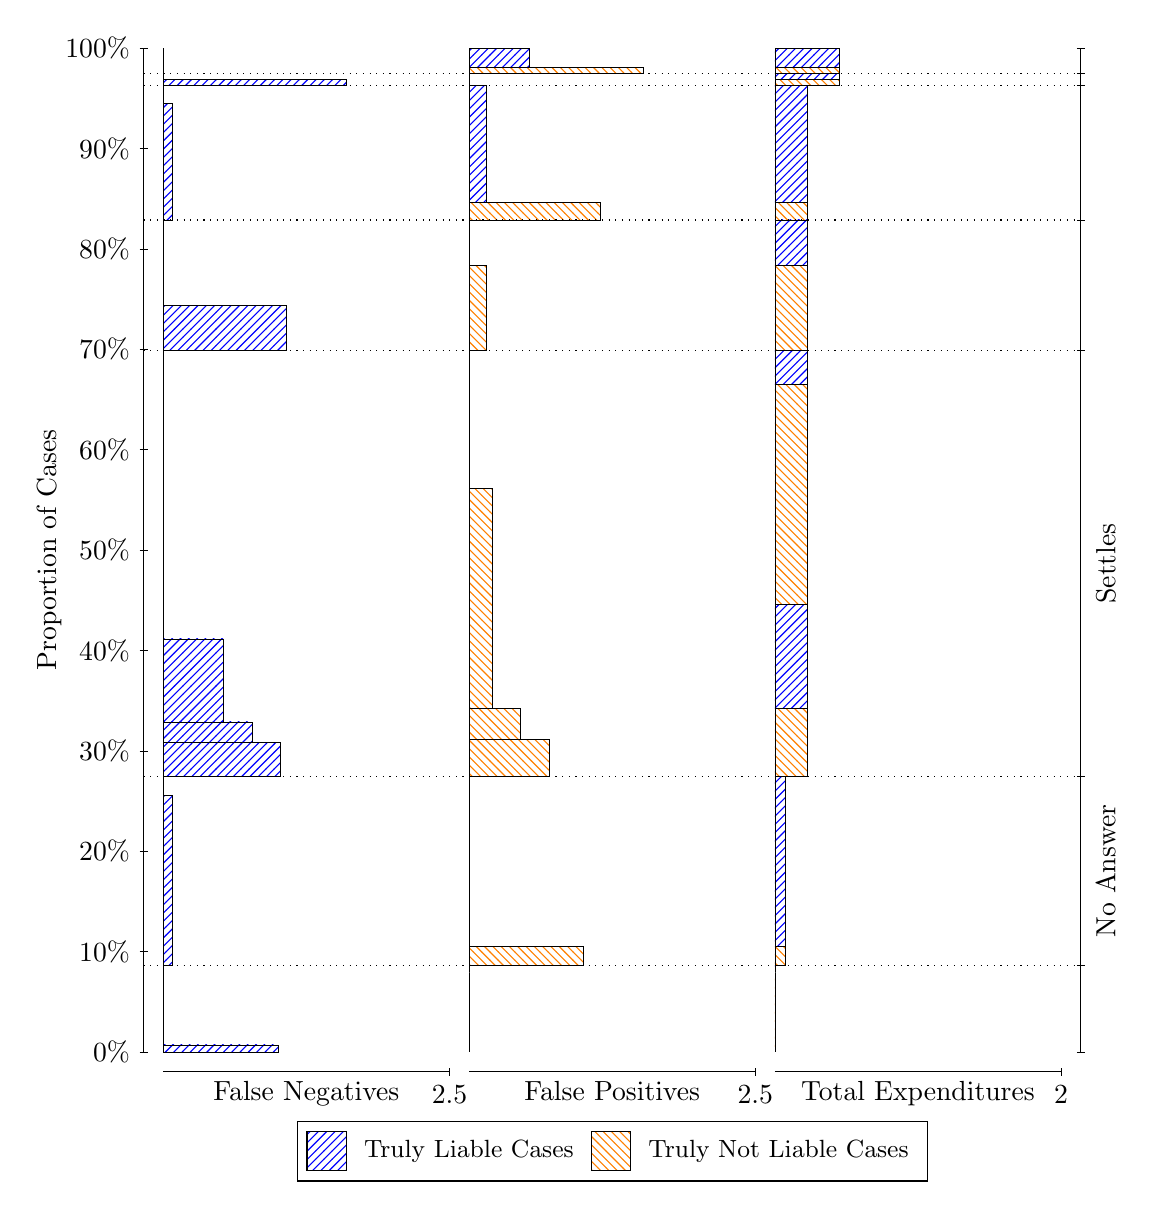
\begin{tikzpicture}
\draw[black, very thin] (1.5,1.75) -- (1.5,14.5);
\node[rotate=90, text=black, anchor=center] at (0.3, 8.125) {Proportion of Cases};
\draw[black, very thin] (1.45,1.75) -- (1.55,1.75);
\node[text=black, anchor=east] at (1.45, 1.75) {0\%};
\draw[black, very thin] (1.45,3.025) -- (1.55,3.025);
\node[text=black, anchor=east] at (1.45, 3.025) {10\%};
\draw[black, very thin] (1.45,4.3) -- (1.55,4.3);
\node[text=black, anchor=east] at (1.45, 4.3) {20\%};
\draw[black, very thin] (1.45,5.575) -- (1.55,5.575);
\node[text=black, anchor=east] at (1.45, 5.575) {30\%};
\draw[black, very thin] (1.45,6.85) -- (1.55,6.85);
\node[text=black, anchor=east] at (1.45, 6.85) {40\%};
\draw[black, very thin] (1.45,8.125) -- (1.55,8.125);
\node[text=black, anchor=east] at (1.45, 8.125) {50\%};
\draw[black, very thin] (1.45,9.4) -- (1.55,9.4);
\node[text=black, anchor=east] at (1.45, 9.4) {60\%};
\draw[black, very thin] (1.45,10.675) -- (1.55,10.675);
\node[text=black, anchor=east] at (1.45, 10.675) {70\%};
\draw[black, very thin] (1.45,11.95) -- (1.55,11.95);
\node[text=black, anchor=east] at (1.45, 11.95) {80\%};
\draw[black, very thin] (1.45,13.225) -- (1.55,13.225);
\node[text=black, anchor=east] at (1.45, 13.225) {90\%};
\draw[black, very thin] (1.45,14.5) -- (1.55,14.5);
\node[text=black, anchor=east] at (1.45, 14.5) {100\%};

\draw[black, very thin] (13.4,1.75) -- (13.4,14.5);
\draw[black, very thin] (13.35,1.75) -- (13.45,1.75);
\node[anchor=west] at (13.35, 1.75) {};
\draw[black, very thin] (13.35,2.8498) -- (13.45,2.8498);
\node[anchor=west] at (13.35, 2.8498) {};
\draw[black, very thin] (13.35,5.2456) -- (13.45,5.2456);
\node[anchor=west] at (13.35, 5.2456) {};
\draw[black, very thin] (13.35,10.661) -- (13.45,10.661);
\node[anchor=west] at (13.35, 10.661) {};
\draw[black, very thin] (13.35,12.316) -- (13.45,12.316);
\node[anchor=west] at (13.35, 12.316) {};
\draw[black, very thin] (13.35,14.021) -- (13.45,14.021);
\node[anchor=west] at (13.35, 14.021) {};
\draw[black, very thin] (13.35,14.182) -- (13.45,14.182);
\node[anchor=west] at (13.35, 14.182) {};
\draw[black, very thin] (13.35,14.5) -- (13.45,14.5);
\node[anchor=west] at (13.35, 14.5) {};

\draw[black, very thin, pattern color=blue, pattern=north east lines] (1.75,1.75) rectangle (3.2033,1.839);
\draw[black, very thin, pattern color=orange, pattern=north west lines] (1.75,1.839) rectangle (1.75,2.8498);
\draw[black, very thin, pattern color=blue, pattern=north east lines] (1.75,2.8498) rectangle (1.859,5.0073);
\draw[black, very thin, pattern color=orange, pattern=north west lines] (1.75,5.0073) rectangle (1.75,5.2456);
\draw[black, very thin, pattern color=blue, pattern=north east lines] (1.75,5.2456) rectangle (3.2397,5.677);
\draw[black, very thin, pattern color=blue, pattern=north east lines] (1.75,5.677) rectangle (2.8763,5.9415);
\draw[black, very thin, pattern color=blue, pattern=north east lines] (1.75,5.9415) rectangle (2.513,6.9957);
\draw[black, very thin, pattern color=orange, pattern=north west lines] (1.75,6.9957) rectangle (1.75,10.661);
\draw[black, very thin, pattern color=blue, pattern=north east lines] (1.75,10.661) rectangle (3.3123,11.236);
\draw[black, very thin, pattern color=orange, pattern=north west lines] (1.75,11.236) rectangle (1.75,12.316);
\draw[black, very thin, pattern color=blue, pattern=north east lines] (1.75,12.316) rectangle (1.859,13.801);
\draw[black, very thin, pattern color=orange, pattern=north west lines] (1.75,13.801) rectangle (1.75,14.021);
\draw[black, very thin, pattern color=blue, pattern=north east lines] (1.75,14.021) rectangle (4.0753,14.098);
\draw[black, very thin, pattern color=orange, pattern=north west lines] (1.75,14.098) rectangle (1.75,14.182);
\draw[black, very thin, pattern color=orange, pattern=north west lines] (1.75,14.182) rectangle (1.75,14.259);
\draw[black, very thin, pattern color=blue, pattern=north east lines] (1.75,14.259) rectangle (1.75,14.5);
\draw[black, very thin, pattern color=orange, pattern=north west lines] (5.6333,1.75) rectangle (5.6333,2.7608);
\draw[black, very thin, pattern color=blue, pattern=north east lines] (5.6333,2.7608) rectangle (5.6333,2.8498);
\draw[black, very thin, pattern color=orange, pattern=north west lines] (5.6333,2.8498) rectangle (7.0867,3.0881);
\draw[black, very thin, pattern color=blue, pattern=north east lines] (5.6333,3.0881) rectangle (5.6333,5.2456);
\draw[black, very thin, pattern color=orange, pattern=north west lines] (5.6333,5.2456) rectangle (6.6507,5.7206);
\draw[black, very thin, pattern color=orange, pattern=north west lines] (5.6333,5.7206) rectangle (6.2873,6.1152);
\draw[black, very thin, pattern color=orange, pattern=north west lines] (5.6333,6.1152) rectangle (5.924,8.9105);
\draw[black, very thin, pattern color=blue, pattern=north east lines] (5.6333,8.9105) rectangle (5.6333,10.661);
\draw[black, very thin, pattern color=orange, pattern=north west lines] (5.6333,10.661) rectangle (5.8513,11.741);
\draw[black, very thin, pattern color=blue, pattern=north east lines] (5.6333,11.741) rectangle (5.6333,12.316);
\draw[black, very thin, pattern color=orange, pattern=north west lines] (5.6333,12.316) rectangle (7.3047,12.536);
\draw[black, very thin, pattern color=blue, pattern=north east lines] (5.6333,12.536) rectangle (5.8513,14.021);
\draw[black, very thin, pattern color=orange, pattern=north west lines] (5.6333,14.021) rectangle (5.6333,14.105);
\draw[black, very thin, pattern color=blue, pattern=north east lines] (5.6333,14.105) rectangle (5.6333,14.182);
\draw[black, very thin, pattern color=orange, pattern=north west lines] (5.6333,14.182) rectangle (7.8497,14.259);
\draw[black, very thin, pattern color=blue, pattern=north east lines] (5.6333,14.259) rectangle (6.3963,14.5);
\draw[black, very thin, pattern color=orange, pattern=north west lines] (9.5167,1.75) rectangle (9.5167,2.7608);
\draw[black, very thin, pattern color=blue, pattern=north east lines] (9.5167,2.7608) rectangle (9.5167,2.8498);
\draw[black, very thin, pattern color=orange, pattern=north west lines] (9.5167,2.8498) rectangle (9.6529,3.0881);
\draw[black, very thin, pattern color=blue, pattern=north east lines] (9.5167,3.0881) rectangle (9.6529,5.2456);
\draw[black, very thin, pattern color=orange, pattern=north west lines] (9.5167,5.2456) rectangle (9.9254,6.1152);
\draw[black, very thin, pattern color=blue, pattern=north east lines] (9.5167,6.1152) rectangle (9.9254,7.4339);
\draw[black, very thin, pattern color=orange, pattern=north west lines] (9.5167,7.4339) rectangle (9.9254,10.229);
\draw[black, very thin, pattern color=blue, pattern=north east lines] (9.5167,10.229) rectangle (9.9254,10.661);
\draw[black, very thin, pattern color=orange, pattern=north west lines] (9.5167,10.661) rectangle (9.9254,11.741);
\draw[black, very thin, pattern color=blue, pattern=north east lines] (9.5167,11.741) rectangle (9.9254,12.316);
\draw[black, very thin, pattern color=orange, pattern=north west lines] (9.5167,12.316) rectangle (9.9254,12.536);
\draw[black, very thin, pattern color=blue, pattern=north east lines] (9.5167,12.536) rectangle (9.9254,14.021);
\draw[black, very thin, pattern color=orange, pattern=north west lines] (9.5167,14.021) rectangle (10.334,14.105);
\draw[black, very thin, pattern color=blue, pattern=north east lines] (9.5167,14.105) rectangle (10.334,14.182);
\draw[black, very thin, pattern color=orange, pattern=north west lines] (9.5167,14.182) rectangle (10.334,14.259);
\draw[black, very thin, pattern color=blue, pattern=north east lines] (9.5167,14.259) rectangle (10.334,14.5);
\draw[black, dotted] (1.5,2.8498) -- (13.4,2.8498);
\draw[black, dotted] (1.5,5.2456) -- (13.4,5.2456);
\draw[black, dotted] (1.5,10.661) -- (13.4,10.661);
\draw[black, dotted] (1.5,12.316) -- (13.4,12.316);
\draw[black, dotted] (1.5,14.021) -- (13.4,14.021);
\draw[black, dotted] (1.5,14.182) -- (13.4,14.182);
\draw[black, very thin] (1.75,1.5) -- (5.3833,1.5);
\node[text=black, anchor=north] at (3.5667, 1.5) {False Negatives};
\draw[black, very thin] (5.3833,1.45) -- (5.3833,1.55);
\node[text=black, anchor=north] at (5.3833, 1.45) {2.5};

\draw[black, very thin] (5.6333,1.5) -- (9.2667,1.5);
\node[text=black, anchor=north] at (7.45, 1.5) {False Positives};
\draw[black, very thin] (9.2667,1.45) -- (9.2667,1.55);
\node[text=black, anchor=north] at (9.2667, 1.45) {2.5};

\draw[black, very thin] (9.5167,1.5) -- (13.15,1.5);
\node[text=black, anchor=north] at (11.333, 1.5) {Total Expenditures};
\draw[black, very thin] (13.15,1.45) -- (13.15,1.55);
\node[text=black, anchor=north] at (13.15, 1.45) {2};


\node[text=black, centered, rotate=90] at (13.72, 4.0477) {No Answer};
\node[text=black, centered, rotate=90] at (13.72, 7.9531) {Settles};





\draw (7.449999999999999,1.5) node[draw=none] (baseCoordinate) {};
\begin{scope}[align=center]
        \matrix[scale=0.5, draw=black, below=0.5cm of baseCoordinate, nodes={draw}, column sep=0.1cm]{
            \node[rectangle, draw, minimum width=0.5cm, minimum height=0.5cm, pattern color=blue, pattern=north east lines] {}; &
            \node[draw=none, font=\small, text=black] (B) {Truly Liable Cases}; &
            \node[rectangle, draw, minimum width=0.5cm, minimum height=0.5cm, pattern color=orange, pattern=north west lines] {}; &
            \node[draw=none, font=\small, text=black] (B) {Truly Not Liable Cases}; \\
            };
\end{scope}

\end{tikzpicture}
\end{document}